\chapter{Implementacija i korisničko sučelje}
		
		
		\section{Korištene tehnologije i alati}
		
			\textbf{\textit{dio 2. revizije}}
			
			Backend dio aplikacije pisan je u objektno orijentiranom programskom jeziku  \href{https://www.java.com/en/}{\textbf{Java}}\footnote{https://www.java.com/en/}. Jedna od glavnih značajki ovog jezika je takozvano načelo WORA (eng. \textit{write once, run anywhere}) koje omogućava da se jednom prevedeni kod pomoću Javinog virtualnog stroja može izvršavati na bilo kojem računalu. Jedini preduvjet je da to računalo na sebi ima instaliranu Javinu platformu.
			
			Kako bi se olakšao razvoj backend dijela aplikacije, korišten je radni okvir \href{https://spring.io/projects/spring-boot/}{\textbf{Spring Boot}}\footnote{https://spring.io/projects/spring-boot/} koji je specijalizacija radnog okvira Spring. Spring Boot je popularan radni okvir za izgradnju samostojećih web aplikacija. Glavna prednost ovog radnog okvira je automatska konfiguracija dijelova koda koji se standardno pojavljuju kod web aplikacija. Tako Spring Boot automatizira komunikaciju s bazom podataka, rad s datotekama u JSON formatu, podjela programskog koda u unaprijed definirane slojeve itd.
			
			Backend dio aplikacije je razvijan u razvojnom okruženju \href{https://www.jetbrains.com/idea/}{\textbf{IntelliJ IDEA}}\footnote{https://www.jetbrains.com/idea/} tvrtke JetBrains. Samo razvojno okruženje je namjenjenu razvoju u programskim jezicima Java, Kotlin, Groovy, Scala te je jedno od vodećih okruženja za te programske jezike. IntelliJ IDEA programeru nudi razne funkcionalnosti koje ubrzavaju i olakšavaju programiranje kao što su samozavršavanjne koda analizom konteksta, navigacija u kodu, refaktoriranje koda, debuggiranje, rad sa distribuiranim sustavima za upravljanje verzijama podataka, kao što je Git, rad s bazom podataka itd. Također, IntelliJ IDEA programer može dodatno nadograditi instaliranjem proširenja za dodatne funkcionalnosti koja su dostupna na web repozitoriju JetBrainsa.
			
			Frontend dio aplikacije je pisan u programskom jeziku \href{https://www.javascript.com/}{\textbf{JavaScript}}\footnote{https://www.javascript.com/} koji efektivno postao nezabiolazan jezik za razvoj klijentske strane web aplikacija. JavaScript je dinamičan skriptni jezik sa mekim tipovima podataka (eng. \textit{soft-typed}) kojeg podržava svaki moderan web preglednik. Za sam jezik JavaScript postoji napisano puno javno dostupnih biblioteka koje olakšavaju ostvarivanje raznih funkcionalnosti u kodu i potiču ponovnu uporabu postojećeg koda. Iako je Javascript de facto standard za razvoj frontend dijela aplikacije, također se može koristiti i za razvoj backend dijela aplikacije.
			
			Za brži i lakši razvoj frontend dijela aplikacije korištena je vrlo popularna biblioteka  \href{https://react.dev/}{\textbf{React}}\footnote{https://react.dev/} razvijena od tvrtke Meta (nekada Facebook). Aplikacije napravljene u Reactu koriste komponente koje se mogu koristiti na više mjesta. React koristi virtualni DOM (Document Object Model) te se pomoću Reacta grade jednostranične web aplikacije koje osvježavaju samo komponente koje je potrebno mijenjati. Time se značajno poboljšavaju performanse web aplikacije.
			
			Kako bi dodatno olakšali vizualno oblikovanje korisničkog sučelja korišten je radni okvir \href{https://getbootstrap.com/}{\textbf{Bootstrap}}\footnote{https://getbootstrap.com/}. Bootstrap je popularan radni okvir za stilski jezik CSS koji olakšava vizualno oblikovanje korisničkog sučelja nuđenjem gotovih dizajnova osnovnih elemenata web stranice kao što su na primjer gumbovi, forme i sl. 
			
			Za razvoj frontend dijela aplikacije korišteno je razvojno okruženje \href{https://code.visualstudio.com/}{\textbf{Visual Studio Code}}\footnote{https://code.visualstudio.com/} tvrtke Microsoft. Visual Studio Code je moguće nadograđivati raznim proširenjima pomoću kojih se može stvoriti razvojno okruženje za gotovo svaki programski jezik kao što je C, C++, Java, JavaScript, Python, Go, itd. Zbog te fleksibilnosti se Visual Studio Code može koristiti u gotovo svakoj domeni koja uključuje neku vrstu programiranja.
			
			Baza podataka je napravljena u sustavu \href{https://www.postgresql.org/}{\textbf{PostgreSQL}}\footnote{https://www.postgresql.org/}. PostgreSQL je jedan od najraširenijih sustava za upravljanje relacijskim bazama podataka temeljen na SQL-u (Structured Query Language). PostgreSQL omogućuje izradu baza podataka sa raznim funkcionalnostima kao što su okidači, transakcije, procedure, mogćnost paralelnog pristupa više korisnika istovremeno, konzistencija i sigurnost podataka, itd.
			
			Svi dijagrami za opis sustava napravljeni su u \href{https://www.uml.org/}{\textbf{UML-u}}\footnote{https://www.uml.org/} (Unified Modeling Language). UML je generički jezik za vizualno modeliranje. Napravljen je kako bi pružao standard za dizajniranje sustava. Taj standard omogućava bolju vizualizaciju, specifikaciju, oblikovanje i dokumentiranje artefakata programske potpore. U svrhu vizualizacije pojedinog aspekta sustava definiran je veliki broj vrsta dijagrama koji omogućuju različite poglede na pojedini dio sustava.
			
			Za izradu UML dijagrama korišten je grafički alat \href{https://www.visual-paradigm.com/}{\textbf{Visual Paradigm}}\footnote{https://www.visual-paradigm.com/}. On podržava izradu mnogih vrsta UML dijagrama kao što su dijagram obrazaca uporabe, sekvencijski dijagram, dijagram stanja, dijagram komponenti, dijagram aktivnosti, dijagram razmještaja, dijagram razreda, i mnogi drugi.
			
			Za potrebe izrade dijagrama razreda korištena je funkcionalnost razvojnog okruženja IntelliJ IDEA za automatsko generiranje dijagrama razreda iz postojećeg programskog koda. Dobiveni dijagram razreda je dodatno uređen i dorađen u grafičkom alatu za izradu dijagrama  \href{https://www.drawio.com/}{\textbf{draw.io}}\footnote{https://www.drawio.com/}.
			
			Izrada relacijskog dijagrama baze podataka i modeliranje same baze podataka ostvareno je uz grafički alat \href{https://erdplus.com/}{\textbf{ERDPlus}}\footnote{https://erdplus.com/}. ERDPlus omogućuje izradu ER dijagrama baze podataka koji se sastoji od entiteta i veza između njih. Iz ER dijagrama je moguće automatsko generiranje relacijskih dijagrama baze podataka. Iz dobivenih relacijskih dijagrama je moguće automatsko generiranje SQL naredbi za stvaranje odgovarajućih tablica u bazi podataka.
			
			Dokumentacija je pisana u jeziku \href{https://www.latex-project.org/}{\textbf{LaTeX}}\footnote{https://www.latex-project.org/}. LaTeX je široko korišten jezik za pisanje dokumenata koji pruža široke mogućnosti i omogućuje jednostavniju izradu složenih dokumenata. S obzirom da se radi o markup jeziku, LaTeX omogućuje odvajanje stila od sadržaja što kod složenih dokumenata daje veliku prednost u odnosu na standardne aplikacije za pisanje dokumenata kao što su MS Word.
			
			U svrhu pisanja dokumentacije u LaTeX-u korišten je \href{https://www.texstudio.org/}{\textbf{TeXstudio}}\footnote{https://www.texstudio.org/}. TeXstudio je uređivač teksta posebno napravljen upravo za pisanje dokumenata u jeziku LaTeX.
			
			Za upravljanje programskim kodom, dokumentacijom i ostalim datotekama koje su korištene u ovom projektu korišten je sustav \href{https://git-scm.com/}{\textbf{Git}}\footnote{https://git-scm.com/}. Git je popularan distribuirani sustav za upravljanje verzijama podataka. Izuzetno je koristan kada više ljudi u timu radi na nekom projektu jer omogućuje koordinaciju istovremenog rada više ljudi na projektu. Sastoji se od udaljenog repozitorija, obično na nekoj Git platformi u oblaku, te lokalnih kopija tog repozitorija na računalima korisnika koji sudjeluju u projektu. Git prati kompletnu povijest promjena u repozitoriju i nudi razne mogućnosti koje olakšavaju distribuirani rad.
			
			Kao Git platforma u oblaku je za ovaj projekt korišten \href{https://github.com/}{\textbf{GitHub}}\footnote{https://github.com/}. GitHub je danas najraširenija platforma za spremanje programskih projekata i distribuirani sustav za upravljanje verzijama.
			
			Za puštanje aplikacije i popratne baze podataka u pogon korištena je usluga oblaka \href{https://render.com/}{\textbf{Render}}\footnote{https://render.com/}. Render je sustav u oblaku koji služi za izgradnju i pokretanje raznih programskih sustava, pa tako i web aplikacija i baza podataka. Prednosti Rendera su njegovo lagano integriranje s GitHubom, automatsko deployanje prilikom promjena na grani u Git repozitoriju te postojanje besplatne usluge uz određena ograničenja koja za ovaj projekt nisu pretjerano bitna.
			
			Prilikom puštanja web aplikaacije u pogon korištena je tehnologija \href{https://www.docker.com/}{\textbf{Docker}}\footnote{https://www.docker.com/}. Docker omogućuje jednostavnu izradu kontejnera koji u sebi sadrže neku programsku podršku. Kontejner je oblik virtualizacije na razini operacijskog sustava. Ovim oblikom virtualizacije se stvara okruženje jednostavnije od onog dobivenog virtualnim strojem, ali još uvijek omogućuje da programska podrška u kontejneru bude nezavisna od okruženja na kojem je kontejner pokrenut. Docker kontejner se opisuje posebnom skriptom koja se zove Dockerfile.  
			
			Članovi tima su međusobno komunicirali preko društvenih mreža \href{https://discord.com/}{\textbf{Discord}}\footnote{https://discord.com/} i \href{https://www.messenger.com/}{\textbf{Messenger}}\footnote{https://www.messenger.com/}. Messenger je jednostavna društvena mreža koja kao glavni način komunikacije koristi izmjenu poruka između dva korisnika ili unutar grupe korisnika. Discord je društvena mreža u kojoj korisnici mogu komunicirati porukama, glasovnim pozivima i video pozivima. Korisnici mogu komunicirati unutar širih zajednica koje se nazivaju serveri. Unutar servera postoje tekstualni kanali kao i glasovni kanali za glasovne pozive sa više korisnika.
			
			Za ispitivanje sustava u cjelini korišten je radni okvir \href{https://www.selenium.dev/}{\textbf{Selenium}}\footnote{https://www.selenium.dev/}. Selenium je alat koji služi za testiranje web aplikacija pomoću web preglednika. Skripte za testiranje se mogu pisati u raznim programskim jezicima. 
			
			Za testiranje pojedinih komponenti sustava korišten je radni okvir \href{https://junit.org/junit5/}{\textbf{JUnit}}\footnote{https://junit.org/junit5/}. JUnit je radni okvir koji služi za testiranje funkcionalnosti pojedinih dijelova programskog koda pisanog u programskom jeziku Java.
			
			\eject 
		
	
		\section{Ispitivanje programskog rješenja}
			
			\textbf{\textit{dio 2. revizije}}\\
			
			 \textit{U ovom poglavlju je potrebno opisati provedbu ispitivanja implementiranih funkcionalnosti na razini komponenti i na razini cijelog sustava s prikazom odabranih ispitnih slučajeva. Studenti trebaju ispitati temeljnu funkcionalnost i rubne uvjete.}
	
			
			\subsection{Ispitivanje komponenti}
			\textit{Potrebno je provesti ispitivanje jedinica (engl. unit testing) nad razredima koji implementiraju temeljne funkcionalnosti. Razraditi \textbf{minimalno 6 ispitnih slučajeva} u kojima će se ispitati redovni slučajevi, rubni uvjeti te izazivanje pogreške (engl. exception throwing). Poželjno je stvoriti i ispitni slučaj koji koristi funkcionalnosti koje nisu implementirane. Potrebno je priložiti izvorni kôd svih ispitnih slučajeva te prikaz rezultata izvođenja ispita u razvojnom okruženju (prolaz/pad ispita). }
			
			
			
			\subsection{Ispitivanje sustava}
			
			 \textit{Potrebno je provesti i opisati ispitivanje sustava koristeći radni okvir Selenium\footnote{\url{https://www.seleniumhq.org/}}. Razraditi \textbf{minimalno 4 ispitna slučaja} u kojima će se ispitati redovni slučajevi, rubni uvjeti te poziv funkcionalnosti koja nije implementirana/izaziva pogrešku kako bi se vidjelo na koji način sustav reagira kada nešto nije u potpunosti ostvareno. Ispitni slučaj se treba sastojati od ulaza (npr. korisničko ime i lozinka), očekivanog izlaza ili rezultata, koraka ispitivanja i dobivenog izlaza ili rezultata.\\ }
			 
			 \textit{Izradu ispitnih slučajeva pomoću radnog okvira Selenium moguće je provesti pomoću jednog od sljedeća dva alata:}
			 \begin{itemize}
			 	\item \textit{dodatak za preglednik \textbf{Selenium IDE} - snimanje korisnikovih akcija radi automatskog ponavljanja ispita	}
			 	\item \textit{\textbf{Selenium WebDriver} - podrška za pisanje ispita u jezicima Java, C\#, PHP koristeći posebno programsko sučelje.}
			 \end{itemize}
		 	\textit{Detalji o korištenju alata Selenium bit će prikazani na posebnom predavanju tijekom semestra.}
			
			\eject 
		
		
		\section{Dijagram razmještaja}
			
			\textbf{\textit{dio 2. revizije}}
			
			Dijagram razmještaja je statički strukturni dijagram koji opisuje topologiju sutava i usredotočen je na odnos sklopovskih i programskih dijelova. Osnovni elementi dijagrama su čvorovi, artefakti i spojevi.
			
			Dijagram \ref{fig:dijagramRazmjestaja} prikazuje topologiju sustava za prijavljivanje oštećenja na javnim površinama. Sustav je napravljen na temelju arhitekture klijent-poslužitelj u kojoj klijent i poslužitelj komuniciraju HTTPS protokolom. Sustav je stavljen u pogon pomoću dva odvojena servisa na usluzi Render, jedan za aplikaciju i jedan za bazu podataka. Na Render servisu za bazu podataka postoji instanca PostgreSQL baze podataka te taj servis prima zahtjeve za bazu podataka na standardnom portu 5432. Na Render servisu za web aplikaciju je pokrenut Docker kontejner unutar kojeg su upogonjeni React frontend i Spring Boot backend dijelovi aplikacije. Spring Boot backend po potrebi komunicira sa bazom podataka slanjem SQL querryja na port 5432 Render servisa za bazu podataka. Render servis za web aplikaciju sluša HTTPS zahtjeve na portu 443. Zaprimljene HTTPS zahtjeve Render servis prosljeđuje na port 8080 Docker kontejnera kao HTTP zahtjeve. Klijentski uređaj na sebi ima pokrenuti web preglednik pomoću kojeg šalje HTTPS zahtjeve na port 443 Render servisa za web aplikaciju.
			
			\begin{figure}[H]
				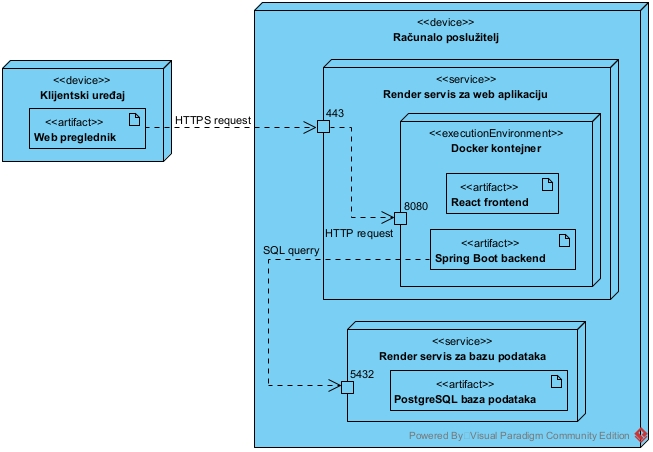
\includegraphics[width=\textwidth]{slike/dijagramRazmjestaja.jpg} %veličina u odnosu na širinu linije
				\caption{Dijagram razmještaja}
				\label{fig:dijagramRazmjestaja} %label mora biti drugaciji za svaku sliku
			\end{figure}
			
			\eject 
		
		\section{Upute za puštanje u pogon}
		
			\textbf{\textit{dio 2. revizije}}\\
			
			 \textit{U ovom poglavlju potrebno je dati upute za puštanje u pogon (engl. deployment) ostvarene aplikacije. Na primjer, za web aplikacije, opisati postupak kojim se od izvornog kôda dolazi do potpuno postavljene baze podataka i poslužitelja koji odgovara na upite korisnika. Za mobilnu aplikaciju, postupak kojim se aplikacija izgradi, te postavi na neku od trgovina. Za stolnu (engl. desktop) aplikaciju, postupak kojim se aplikacija instalira na računalo. Ukoliko mobilne i stolne aplikacije komuniciraju s poslužiteljem i/ili bazom podataka, opisati i postupak njihovog postavljanja. Pri izradi uputa preporučuje se \textbf{naglasiti korake instalacije uporabom natuknica} te koristiti što je više moguće \textbf{slike ekrana} (engl. screenshots) kako bi upute bile jasne i jednostavne za slijediti.}
			
			
			 \textit{Dovršenu aplikaciju potrebno je pokrenuti na javno dostupnom poslužitelju. Studentima se preporuča korištenje neke od sljedećih besplatnih usluga: \href{https://aws.amazon.com/}{Amazon AWS}, \href{https://azure.microsoft.com/en-us/}{Microsoft Azure} ili \href{https://www.heroku.com/}{Heroku}. Mobilne aplikacije trebaju biti objavljene na F-Droid, Google Play ili Amazon App trgovini.}
				
			\eject 